% Lists frame
\section{DMC}
\begin{frame}{Wielowymiarowy DMC}
Schemat projektowania wielowymiarwego algorytmu DMC:
\begin{itemize}
    \item Wyznaczenie wielowymiarowej odpowiedzi skokowej 
    \item Wyznaczenie wektora zmiennych decyzyjnych
    \item Wyznaczenie macierzy wagowych
    \item Wyznaczenie wektora optymalnych przyrostów sterowań
\end{itemize}
Wszystkie sygnały sterujące wpływają na sygnały wyjściowe. 
\end{frame}


\begin{frame}{Wielowymiarowy DMC}
Wyznaczenie wielowymiarowej odpowiedzi skokowej:
	\begin{center}
		\begin{figure}[H]
            		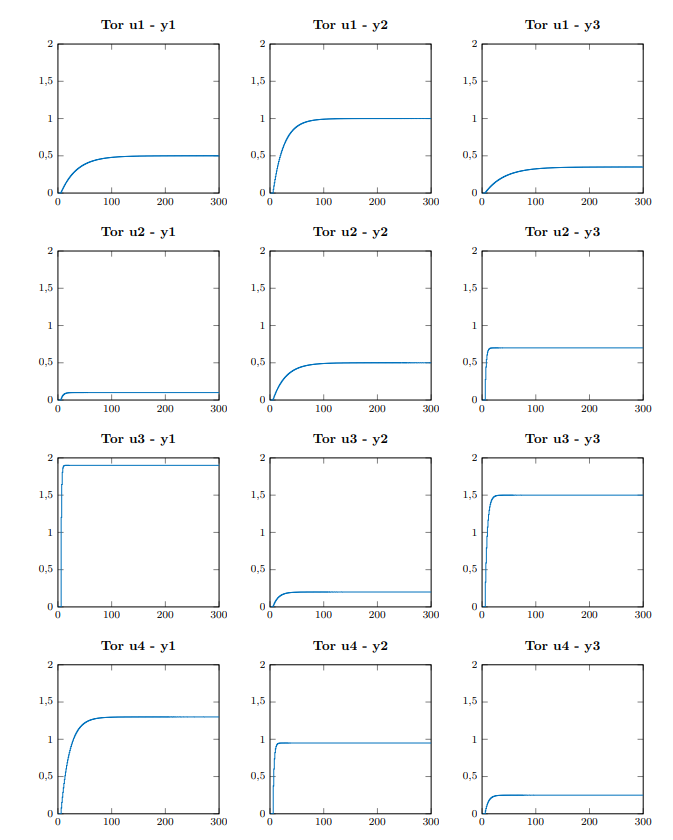
\includegraphics[scale=0.25]{images/PIDtory.png}
          			 \caption{Wielowymiarowa odpowiedź skokowa}
		\end{figure}
	\end{center}
\end{frame}

\begin{frame}{Wielowymiarowy DMC}
Określenie pętli regulacji:
	\begin{center}
		\begin{figure}[H]
            		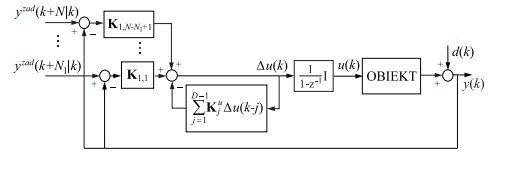
\includegraphics[scale=0.7]{images/SISODMC.png}
          			 \caption{Schemat układu regulacji}
		\end{figure}
	\end{center}
\end{frame}

\begin{frame}{Wielowymiarowy DMC}
Wyniki działania:
	\begin{center}
		\begin{figure}[H]
            		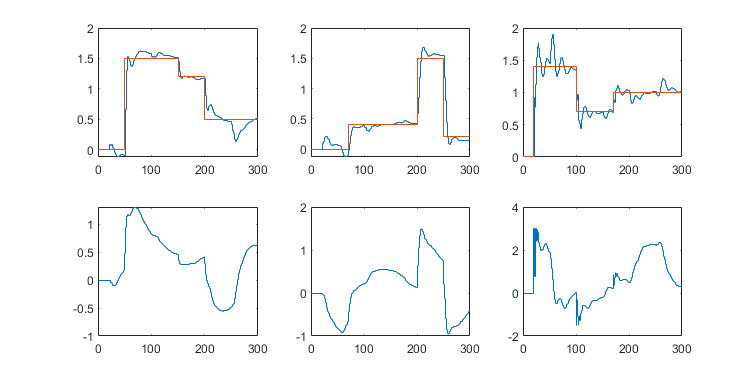
\includegraphics[scale=0.5]{images/PID_wyniki.png} %%do poprawy jak już będą ładne
          			 \caption{Wyniki regulacji}
		\end{figure}
	\end{center}
\end{frame}
